\section{Trifocal Tensor}
\subsection{Tensor Notation}
Tensors are geometric objects used to represent linear relations between vectors, scalars, and other tensors \cite{weisstein1}. A tensor can be represented as a multi-dimensional array of numerical values. The order of a tensor is the dimensionality of the array needed to represent it. Scalars are single numbers and are thus 0th-order tensors. Vectors are 1-dimensional array, 1st-order tensors arranged in a column or row. Matrices are 2-dimensional arrays, 2nd-order tensors arranged as a 2D array of numbers. Similarly, a tensor with three indices may be thought as a 3D array of numbers.

Tensors provide a natural and concise mathematical framework for formulating and solving problems in areas of physics. Tensors express the relationship between vectors, hence they are independent of a particular choice of coordinate system.

The notation for a tensor is similar to that of a matrix, except that a tensor may have an arbitrary number of indices \textit{e.g.:}$A_{ijk\dotsb}$. In addition, a tensor with rank $r+s$ may be of mixed type $(r,s)$, consisting of $r$ \texttt{contravariant (upper)} indices and $s$ \texttt{covariant (lower)} indices. In tensor notation, a vector $v$ would be written $v_i$, where $i =1,\dotsb,m$, and a matrix is a tensor of type $(1,1)$ would be written as $A^{j}_{i}$.

Tensor notation can provide a very concise way of writing vector and more general identities. For example, the dot product $u.v$ can be simply written as
$$
u.v = u_{i}v^{i}
$$
where repeated indices are summed over. This is called \texttt{Einstein Summation} \cite{weisstein2}. It is a notational convention for simplifying expressions including summations of vectors, matrices and general tensors. The convention can be best illustrated through the following equation
$$
  c^{i}_{k} = a^{i}_{j}b^{j}_{k} = \sum_{j} a_{ij}b_{jk}
$$

Similarly, the cross product can be concisely written as
$$
  (u\times v)_{i} = \epsilon_{ijk} u^{j} v^{k},
$$
where $\epsilon_{ijk}$ is the permutation tensor defined for $r,s,t =1,\dotsb,3$ as follows:
$$
\epsilon_{rst} = \begin{cases}
  0 & \text{ unless } r,s \text{ and } t \text{ are distinct}\\
  +1 & \text{ if } rst \text{ is an even permutation of } 123\\
  -1 & \text{ if } rst \text{ is an odd permutation of } 123
\end{cases}
$$

\subsection{Three-View Geometry}
The Trifocal Tensor is a $3 \times 3 \times 3$ array of numbers that incorporates all projective geometric relationships among three views \cite{Hartley2004}. It relates the coordinates of corresponding points or lines in three views, being independent of the scene structure and depending only on the relative motion among the three views and their intrinsic calibration parameters. Hence, the trifocal tensor can be considered as the generalization of the fundamental matrix in three views. It can also be seen as a collection of three rank-two $3 \times 3$ matrices $T_1, T_2, T_3$.

The geometric basis for the trifocal tensor can be deduced from the incidence relationship of three corresponding lines. We start by supposing a line 3-space is imaged in three views as in Figure.\ref{fig:threeviews}.

The planes back-projected from the lines in each view must all meet in a single line in space, the 3D line that projects to the mated line in the three images. Since in general three arbitrary planes in space do not meet in a single line, this geometric incidence condition provides a genuine constraint on sets of corresponding lines.

\begin{figure}[ht!]
  \centering
  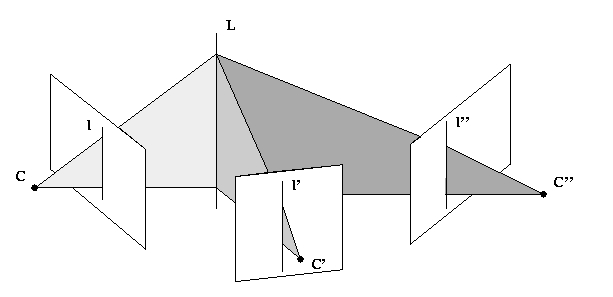
\includegraphics[width=100mm]{figures/threeviews.jpg}
  \caption{Trifocal geometry of three views}
  \label{fig:threeviews}
\end{figure}

Let $ l_i \leftrightarrow l^{\prime}_i \leftrightarrow l^{\prime \prime}_i $ be the set of corresponding lines of $L$. Let the camera matrices for the three views be $P =  \begin{bmatrix} I \mid 0 \end{bmatrix}$, $P^{\prime} = \begin{bmatrix} A \mid a_{4} \end{bmatrix}$, $P^{\prime \prime} = \begin{bmatrix} B \mid b_{4} \end{bmatrix}$, where $A$ and $B$ are $3 \times 3$ matrices, and the vectors $a_i$ and $b_i$ are the \texttt{i}-th columns of the respective camera matrices for $i = 1,\dotsb,4$. $A$ and $B$ are the homographies from the first to the second and third cameras respectively. Due to our choice for the first camera matrix, $a_4$ and $b_4$ are consequently the epipoles of the first camera in views two and three respectively.
 \begin{align*}
  a_4 &= e^{\prime} = P^{\prime}C  & b_4 &= e^{\prime \prime}  = P^{\prime \prime}C
 \end{align*}

Each image line back-projects to a plane as shown in Figure.\ref{fig:threeviews}. These planes are
\begin{align*}
\pi &= P^{T}l = \begin{pmatrix} l \\ 0 \end{pmatrix}  & \pi^{\prime} &= P^{\prime T}l^{\prime} = \begin{pmatrix} A^{T}l^{\prime} \\ a^{T}_{4}l^{\prime} \end{pmatrix} & \pi^{\prime \prime} &= P^{\prime \prime T}l^{\prime \prime} = \begin{pmatrix} B^{T}l^{\prime \prime} \\ b^{T}_{4}l^{\prime \prime} \end{pmatrix}
\end{align*}

The intersection constraint of the three planes in the common line in 3-space can be expressed algebraically by the requirement that the $4 \times 3$ matrix $ M = \begin{bmatrix} \pi & \pi^{\prime} & \pi^{\prime \prime} \end{bmatrix}$ has rank $2$. Points on the line of intersection may be represented as $X = \alpha X_1 + \beta X_2$, with $X_1$ and $X_2$ linearly independent. Such points lie on all three planes and so $\pi^{T}X = \pi^{\prime T}X = \pi^{\prime \prime T}X = 0$. It follows that $M^{T}X = 0$. Consequently M has a 2-dimensional null-space since $M^{T}X_1 = 0$ and $M^{T}X_2 =0$.

Since the rank of $M$ is 2, there is a linear dependence between its columns $m_i$, such that.
\begin{gather*}
M = \begin{bmatrix} m_1, m_2,m_3 \end{bmatrix} = \begin{bmatrix} l & A^{T}l^{\prime} & B^{T}l^{\prime \prime} \\
  0 & a^{T}_{4}l^{\prime} & b^{T}_{4}l^{\prime \prime}
\end{bmatrix}\\
m_1 = \alpha m_2 + \beta m_3
\end{gather*}

From the 2nd row of $M$, $\alpha = k(b^{T}_4 l^{\prime \prime})$ and $\beta = -k(a^{T}_4 l^{\prime})$ for some scalar $k$. Applying this back to the 1st row get
\begin{gather*}
l = (b^{T}_4 l^{\prime \prime })A^{T}l^{\prime} - (a^{T}_4 l^{\prime})B^{T}l^{\prime \prime}\\
l = (l^{\prime \prime T} b_{4})A^{T}l^{\prime} - (l^{\prime T} a_{4})B^{T}l^{\prime \prime}
\end{gather*}

The \texttt{i}-th coordinate $l_i$ of $l$ may be written as
\begin{gather*}
  l_i = l^{\prime \prime T} (b_{4}a^{T}_{i}) l^{\prime} - l^{\prime T}(a_{4}b^{T}_{i}) l^{\prime \prime}\\
  l_i = l^{\prime T} (a_{i}b^{T}_{4}) l^{\prime \prime} - l^{\prime T}(a_{4}b^{T}_{i}) l^{\prime \prime}
\end{gather*}

This relationship can be expressed with the permutation tensor such as
\begin{gather}
  \mathcal{T}_{i} = a_{i}b^{T}_{4} - a_{4}b^{T}_{i} \label{eq:trifocalgeometry1}\\
  l_i = l^{\prime T} \mathcal{T}_{i} l^{\prime \prime} \label{eq:trifocalgeometry2}
\end{gather}

$\mathcal{T}$ is then the trifocal tensor relating the 3 views together. It has 27 elements. There are 26 independent rations apart from the common overall scaling factor of the tensor. However, the tensor has only 18 independent degrees of freedom. Each of 3 camera matrices has 11 degrees of freedom which makes $33$ in total. However, $15$ degrees of freedom must be subtracted to account for the projective world frame, thus leaving 18 degrees of freedom.

\begin{figure}[ht!]
  \centering
  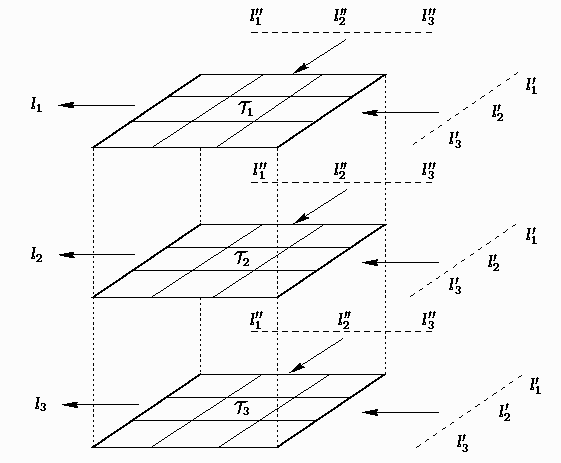
\includegraphics[width=100mm]{figures/trifocaltensor.png}
  \caption{A 3D representation of the trifocal tensor $l_{i} = l_{j}^{\prime} l_{k}^{\prime \prime} \mathcal{T}_{i}^{jk}$ }
  \label{fig:trifocaltensor}
\end{figure}

A point $x$ on the line $l$ must satisfy $x^{T}l = \sum_{i} x^{i}l_{i} = 0$. From \eqref{eq:trifocalgeometry2}, this may be written as
$
l^{\prime T}(\sum_{i} x^{i}\mathcal{T}_{i}) l^{\prime \prime} = 0
$
which means that there exists a 3D point $X$ mapping to $x$ in the first image, and to points on the lines $l^{\prime}$ and $l^{\prime \prime}$ in the second and third images. It's the incidence relationship that holds point-line-line correspondence.

To develop the point-point-point correspondence relationship, we can explore the homography map between the points on first and third images given by $x^{\prime \prime} = Hx$ and $l = H^{T}l^{\prime \prime}$. Thus we get
$$
  h_i = \mathcal{T}^{T}_{i}l^{\prime}
$$
Similarly, the homography from the first to the second views
$$
  h_i = \mathcal{T}_{i}l^{\prime \prime}
$$

Using these results back to our point-line-line correspondence relation,
\begin{gather*}
  x^{\prime \prime} = (\sum_{i} x^{i}\mathcal{T}^{T}_{i}) l^{\prime}
  x^{\prime \prime T}[x^{\prime \prime}]_{\times} = l^{\prime T} (\sum_{i} x^{i}\mathcal{T}_{i})[x^{\prime \prime}]_{\times} = 0^{T}
\end{gather*}

The line $l^{\prime}$ passes through $x^{\prime}$ may be written as $l^{\prime} = [x^{\prime}]_{\times}y^{\prime}$ for some point $y^{\prime}$ on $l^{\prime}$. Then
$$
  y^{\prime T} [x^{\prime}]_{times} (\sum_{i} x^{i}\mathcal{T}_{i})[x^{\prime \prime}]_{\times} = 0^{T}
$$

This relation holds true for all lines $l^{\prime}$ through $x^{\prime}$ and so is independent of $y^{\prime}$, hence this relation can be written as
$$
[x^{\prime}]_{times} (\sum_{i} x^{i}\mathcal{T}_{i})[x^{\prime \prime}]_{\times} = 0_{3\times 3}
$$
which expresses the point-point-point coincidence relationship required. Expressing this relation in proper tensor notation is then given by
\begin{equation}
  x^{i}(x^{\prime j} \epsilon_{jpr})(x^{\prime \prime k} \epsilon_{kqs})\mathcal{T}^{pq}_{i} = 0_{rs} \label{eq:trifocalgeometry3}
\end{equation}

\subsection{Recovering Projection Matrices}
\label{sub:recovering_projection_matrices}
Since the trifocal tensor embeds the geometry of the three cameras in our scene, this implies that the camera matrices may be computed from the trifocal tensor up to a projective ambiguity~\cite{Hartley2004}.

First, the epipoles $e^{\prime},e^{\prime \prime}$ are retrieved. Let $u_i$ and $v_i$ be the left and right null-vectors respectively of $\mathcal{T}_{i}$, \textit{i.e.:} $u_{i}^{T} \mathcal{T}_{i} = {\bf 0}^{T}, \mathcal{T}_{i}v_i = 0$. Then the epipoles are obtained as the null vectors to the following $ 3 \times 3$ matrices:
\begin{equation}
  e^{\prime T} [u_1, u_2, u_3] = 0  \text{ and } e^{\prime \prime T}[v_1, v_2, v_3] = 0
  \label{eq:recoveringepipoles}
\end{equation}

Next, to retrieve the camera matrices $P^{\prime}, P^{\prime \prime}$. The epipoles are normalized to unit norm, then:
\begin{equation}
  P^{\prime} = [[\mathcal{T}_{1}, \mathcal{T}_{2},\mathcal{T}_{3}] e^{\prime \prime} | e^{\prime}] \text{ and } P^{\prime \prime} = [(e^{\prime \prime} e^{\prime \prime T} - I)[\mathcal{T}_{1}^{T}, \mathcal{T}_{2}^{T},\mathcal{T}_{3}^{T}] e^{\prime} | e^{\prime \prime}]
\end{equation}

\subsection{Estimating Trifocal Tensor}
The trifocal tensor can be computed from feature correspondences across the three views. Computation of tensor using correspondences of points or lines has been studied extensively in literature. The main linear algorithm presented by \texttt{Hartley}\cite{Hartley2004} is the straightforward method to compute the tensor. Other methods make use of \texttt{RANSAC} (RANdom SAmple Consensus) to enable the tensor estimation to be robust to outliers that usually cause the linear algebraic method to fail \cite{torr1997robust}.

Each triplet of corresponding image points gives 4 equations linearly independent. Therefore, a minimum set of 7 correspondences of points are needed for the trifocal tensor computation to uniquely determine the 27 entries of the tensor matrix. Given $n$ point correspondences, let $A$ be a matrix of size $4n \times 27$ and $t$ a vector containing all entires of the tensor, then we have
\begin{equation}
  At = 0
  \label{eq:tensorsvd}
\end{equation}
By applying the least square method or SVD, the tensor is obtained from the solution to this linear system. However, \texttt{Hartley} has shown that this kind of algorithm does not do well if all the points are of the form $(x_1, x_2, 1)$ in homogeneous coordinates with $x_1$ and $x_2$ very much larger than $1$. Therefore, it is necessary to normalize the points of each image separately before computing the tensor. The points are translated in each image so that the centroid of all measured points is at the origin of the image coordinates, and then scaled so that the average distance of a point from the origin is $\sqrt{2}$ units. This way the average point will be something like $(1, 1 ,1)$ in homogeneous coordinates, and each of the homogeneous coordinate will be approximately of equal weight. This transformation improves the condition of the matrix of equations and leads to a better solution. Consequently, a de-normalization step is needed in order to work with the original image coordinates.

This method still suffers from two issues
\begin{enumerate}
  \item The tensor is parameterized by all its entries and this does not take into account the tensor geometrical constraints. Therefore, there is always a risk of obtaining an invalid tensor.
  \item Using all available point correspondences causes the tensor to be significantly affected by the presence of strong outliers.
\end{enumerate}

Hence, an algebraic minimization is needed there after, to use the linear solution as an initial estimate and re-parameterize it by the 24 entries of the projection matrices $P^\prime$ and $P^{\prime \prime}$. The desired tensor is found by minimizing the residual error. The overall procedure is briefly explained here.
\begin{enumerate}
  \item Normalize the set of point triplets by performing transformations $H$, $H^{\prime}$ and $H^{\prime \prime}$. Here $\hat{x} = Hx$, $\hat{x}^{\prime} = H^{\prime}x^{\prime}$, $\hat{x}^{\prime \prime} = H^{\prime \prime} x^{\prime \prime}$.
  \item Compute the tensor linearly by solving a set of equations of the form $At = 0$, where $A$ expresses~\ref{eq:trifocalgeometry3}, and $t$ is the vector of entries of the tensor.
  \item De-normalize the tensor by $T_i = H^{\prime -1} \sum_{j}(H^{T}(i,j)T_j)H^{\prime \prime -T}$
  \item Find the two epipoles $e^{\prime}$ and $e^{\prime \prime}$ from the tensor using~\ref{eq:recoveringepipoles}.
  \item According to Equation~\ref{eq:trifocalgeometry1}, construct the $28 \times 12$ matrix $E$ such that $t = Ea$, where $a$ is the vector representing entries of $a_i$ and $b_i$.
  \item Compute the tensor by minimizing the algebraic error $AEa$ subject to $Ea = 1$.
\end{enumerate}

The above algorithm leads to a geometrically valid tensor because its entries satisfies the equation~\ref{eq:trifocalgeometry1}. However, the main weakness of the algebraic minimization method is that all point correspondences are involved in the tensor computation and still suffers from outliers in practice.
